\documentclass[tikz,border=2mm]{standalone}
\usepackage{tikz}
\usetikzlibrary{decorations.pathmorphing}
\usetikzlibrary{arrows}
\newcommand{\midarrow}{\tikz \draw[-triangle 45] (0,0) -- +(.1,0);}
\newcommand{\altarrow}{\tikz \draw[-triangle 45] (0,0) -- +(.5,0);}


\usetikzlibrary{decorations.markings,calc,arrows.meta}
% Arrow helper


\begin{document}

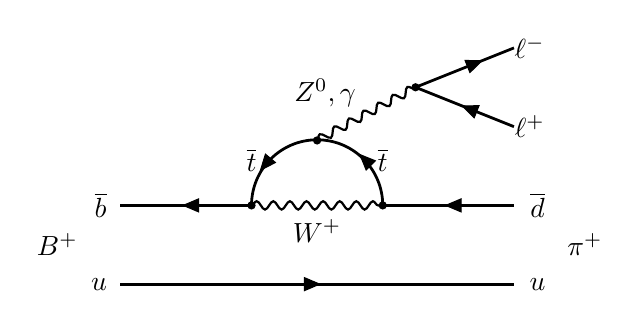
\begin{tikzpicture}[decoration={snake,amplitude=1.5pt,segment length=6pt}]
  % Parameters

\def\L{2.5}      % horizontal radius
\def\H{0.5}

 \coordinate (L1) at (-\L, \H);
 \coordinate (L2) at (-\L, -\H);
 \coordinate (R1) at (\L, \H);
 \coordinate (R2) at (\L, -\H);
 \coordinate (C1) at (-\L/3, \H);
 \coordinate (C2) at (\L/3, \H);
 \coordinate (lept1) at (\L, \H*5);
 \coordinate (lept2) at (\L, \H*3);
 
 \coordinate (J) at (0, \H*2.65);
 \coordinate (JJ) at (\L/2,4*\H);

  \begin{scope}[very thick, every node/.style={sloped,allow upside down}]  
    \draw[line width = 1pt] (L2) -- node {\midarrow} (R2);
    \draw[line width = 1pt] (C1) -- node {\midarrow} (L1);
    \draw[line width = 1pt] (R1) -- node {\midarrow} (C2);
    \draw[line width = 1pt] (JJ) -- node {\altarrow} (lept1);
    \draw[line width = 1pt] (lept2) -- node {\midarrow} (JJ);
    \draw[-triangle 45, rotate = 45+185, line width=0.4pt] ($(C1) + (0-0.5,\H-0.70)$) -- +(0.1,0);
    \draw[-triangle 45, rotate = 135, line width=0.4pt] ($(C1) + (0-0.6,\H-1.93)$) -- +(0.1,0);
  \end{scope}
  % Coordinates
 
  % Upper arc: R -> L (flowing left)
  \draw[line width=1pt] ($(-\L/3,\H)$) arc[start angle=180,end angle=90,x radius=\L/3,y radius=\L/3];
  \draw[line width=1pt] ($(\L/3,\H)$) arc[start angle=0,end angle=90,x radius=\L/3,y radius=\L/3];

  % Endpoints
  %\node[font=\Large\bfseries] at (J) {$\otimes$};
  \draw[decorate,thick] (J) -- (JJ);
  \draw[decorate,thick] (C1) -- (C2);
  %\draw ($\H$) arc (180:0:$\L/3$);
  %\begin{scope}
  %  \fill[white] (J) circle (4.4pt);   % solid white background
  %  \draw[thick] (J) circle (4.4pt);   % circle outline
  %  \node[font=\Large\bfseries] at (J) {$\times$};
    %\draw[thick] (2-4pt,0-4pt) -- (2+4pt,0+4pt); % cross
    %\draw[thick] (2-4pt,0+4pt) -- (2+4pt,0-4pt);
  %\end{scope}

  %\fill (L1) circle (1.5pt);
  %\fill (L2) circle (1.5pt);
  %\fill (R1) circle (1.5pt);
  %\fill (R2) circle (1.5pt);
  \fill (J) circle (1.5pt);
  \fill (JJ) circle (1.5pt);
  \fill (C1) circle (1.5pt);
  \fill (C2) circle (1.5pt);

\node[black] at ($(L1) + (-0.25,0)$) {$\overline{b}$};
\node[black] at ($(L2) + (-0.27,0)$) {$u$};
\node[black] at ($(-\L + (-0.8,0)$) {$B^+$};
%\node[font=\huge] at ($(-\L + (-0.7,0)$) {$\{$};

\node[black] at ($(R1) + (0.3,0)$) {$\overline{d}$};
\node[black] at ($(R2) + (0.30,0)$) {$u$};
\node[black] at ($(\L + (0.9,0)$) {$\pi^+$};
%\node[font=\huge] at ($(\L + (0.7,0)$) {$\}$};

\node[black] at ($(J) + (0.1,0.6)$) {$Z^0,\gamma$};
\node[black] at ($(J) + (0,-\H*2.3)$) {$W^+$};
\node[black] at ($(C1) + (0,\H*1.15)$) {$\overline{t}$};
\node[black] at ($(C2) + (0,\H*1.15)$) {$\overline{t}$};
%\node[font=\small] at ($(J) + (0,-0.25)$) {$V_{ub}$};

\node[black] at ($(lept1) + (0.2,0)$) {$\ell^-$};
\node[black] at ($(lept2) + (0.2,0)$) {$\ell^+$};


  %\node[blue] at ($(S)+(-0.2,0)$) {$J$};
  %\node[blue] at ($(T)+(0.2,0)$) {$h$};
  %\node[red] at ($(Talt)+(0.2,0)$) {$l$};
  %\node[blue] at ($(B)+(0.2,0)$) {$l$};
  %\node[red] at ($(Balt)+(0.2,0)$) {$l$};

  \end{tikzpicture}
  \end{document}